\begin{problem}{전생했더니 슬라임 연구자였던 건에 대하여 (Easy)}{standard input}{standard output}

안녕? 내 이름은 ntopia!

나는 원래 지구에 살고 있던 평범한 20대 청년이었어. 어느 날 길을 걷다가 괴한의 칼에 찔려
죽어버렸어. 그런데 이게 무슨 일이람! 정신을 차려보니 이세계에 떨어져 버렸지 뭐야.
여기에서 나는 슬라임을 전문으로 연구하는 슬라임 연구자가 되어버린 것 같아.
나는 지금 아주 중요한 연구를 진행하고 있어. 이 연구가 성공하면 나는 내가 살던 세계로
돌아갈 수 있게 될 거야. 이 연구를 도와주지 않겠니?

이곳의 슬라임은 모두 슬라임 에너지라는 것을 갖고 있고 그 양은 2 이상의 자연수로 표현돼.
나는 슬라임을 분할했을 때 슬라임 에너지가 어떻게 변화하는지에 대해 연구하고 있어.

슬라임 분할 과정은 1마리를 분할해서 2마리를 만들어내는 식으로 이루어져.
$K$만큼의 슬라임 에너지를 가진 슬라임이 있었다고 해보자. 이 슬라임을 적절히 분할하면
$A$만큼의 에너지를 갖는 슬라임과
$B$만큼의 에너지를 갖는 슬라임을 만들 수 있고 ($A$, $B$는 2 이상의 자연수),
항상 $K = A \times B$ 를 만족해.
이렇게 분할하다보면 언젠가는 분할이 되지 않는 슬라임도 생기겠지?

그리고 슬라임 분할 기술이 아직 완벽하지 않아서 슬라임을 분할할 때마다
흠집이 하나씩 생기게 돼. 구체적으로, 흠집이 $T$개인 슬라임을 분할하면
흠집이 $T+1$개인 슬라임 2마리가 생기는 것이지.

\begin{center}
  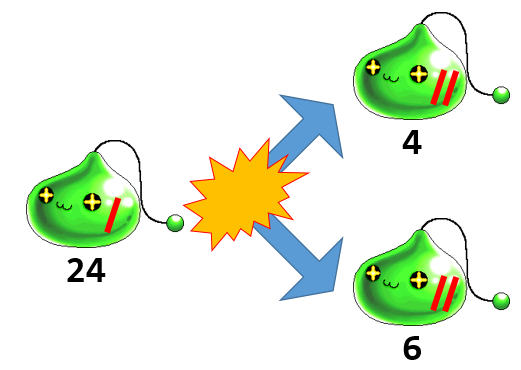
\includegraphics[width=0.7\textwidth]{slime_divide.png}
  \begin{figure}[!h]
  \captionsetup{labelformat=empty,justification=centering}
  \caption{에너지가 24이고 흠집이 1개인 슬라임을 분할한 모습. 에너지가 4이고 흠집이 2개인 슬라임과 에너지가 6이고 흠집이 2개인 슬라임으로 분할되었다.}
  \end{figure}
\end{center}

나에겐 지금 슬라임 에너지가 $K$이고 흠집이 하나도 없는 슬라임이 있어.
이 슬라임을 분할하고 또 분할해서 분할이 가능한 슬라임이 존재하지 않을 때까지 마구마구 분할해야해.
그렇게 다 분할하고나면 마지막에 남은 슬라임들에 흠집이 적당히 생겼겠지?
(물론 생기지 않았을 수도 있어)
그 슬라임들 중에서 흠집이 제일 많이 생긴 녀석의 흠집 개수가 최소가 되도록
분할을 적절히 수행하는 것이 내 연구의 목표야.

내 연구를 도와줘! 부탁이야!!

\InputFile
첫 번째 줄에 처음 주어진 슬라임의 에너지 $K$ ($2 \le K \le 1,000,000$) 가 주어진다.

\OutputFile
슬라임을 끝까지 분할했을 때, 가장 많이 생긴 흠집의 개수의 최솟값을 출력한다.

\Example

\begin{example}
\exmp{10}{1}%
\exmp{3}{0}%
\exmp{24}{2}%
\end{example}

\Notes
처음에 에너지가 24이고 흠집이 없는 슬라임이 있다.
이 슬라임을 에너지가 4인 슬라임과 6인 슬라임으로 분할할 수 있고 각각은 흠집이 1개가 된다.

에너지가 4이고 흠집이 1개인 슬라임은 에너지가 2이고 흠집이 2개인 슬라임 2마리로 분할할 수 있다.

에너지가 6이고 흠집이 1개인 슬라임은 에너지가 2이고 흠집이 2개, 에너지가 3이고 흠집이 2개인 슬라임으로 분할할 수 있다.

이렇게 분할하고 나면 더는 분할이 가능한 슬라임이 존재하지 않게 된다.

이때 가장 많이 생긴 흠집의 개수는 2개이다. 이보다 더 적게 되도록 분할하는 방법은 존재하지 않는다.

\end{problem}
